\documentclass[
	% -- opções da classe memoir --
	12pt,				% tamanho da fonte
	openright,			% capítulos começam em pág ímpar (insere página vazia caso preciso)
	%twoside,			% para impressão em recto e verso. Oposto a oneside
	openany, oneside,
	a4paper,			% tamanho do papel. 
	% -- opções da classe abntex2 --
	%chapter=TITLE,		% títulos de capítulos convertidos em letras maiúsculas
	%section=TITLE,		% títulos de seções convertidos em letras maiúsculas
	%subsection=TITLE,	% títulos de subseções convertidos em letras maiúsculas
	%subsubsection=TITLE,% títulos de subsubseções convertidos em letras maiúsculas
	% -- opções do pacote babel --
	english,			% idioma adicional para hifenização
	brazil				% o último idioma é o principal do documento
	]{abntex2}
	
% ---
% Pacotes básicos 
% ---
\usepackage{lmodern}			% Usa a fonte Latin Modern			
\usepackage[T1]{fontenc}		% Selecao de codigos de fonte.
\usepackage[utf8]{inputenc}		% Codificacao do documento (conversão automática dos acentos)
\usepackage{lastpage}			% Usado pela Ficha catalográfica
\usepackage{indentfirst}		% Indenta o primeiro parágrafo de cada seção.
\usepackage{color}				% Controle das cores
\usepackage{graphicx}			% Inclusão de gráficos
\usepackage{microtype} 			% para melhorias de justificação
\usepackage{fancyvrb}

% ---
		
% ---
% Pacotes adicionais, usados apenas no âmbito do Modelo Canônico do abnteX2
% ---
\usepackage{lipsum}				% para geração de dummy text
% ---

% ---
% Pacotes de citações
% ---
\usepackage[brazilian,hyperpageref]{backref}	 % Paginas com as citações na bibl
\usepackage[alf,abnt-etal-cite=1]{abntex2cite}
% --\usepackage[alf]{abntex2cite}	% Citações padrão ABNT
% -- \citeoption{abnt-etal-cite=2}

% --- 
% CONFIGURAÇÕES DE PACOTES
% --- 

% ---
% Configurações do pacote backref
% Usado sem a opção hyperpageref de backref
\renewcommand{\backrefpagesname}{Citado na(s) página(s):~}
% Texto padrão antes do número das páginas
\renewcommand{\backref}{}
% Define os textos da citação
\renewcommand*{\backrefalt}[4]{
	\ifcase #1 %
		Nenhuma citação no texto.%
	\or
		Citado na página #2.%
	\else
		Citado #1 vezes nas páginas #2.%
	\fi}%
% ---

% ---
% Informações de dados para CAPA e FOLHA DE ROSTO
% ---
\titulo{Busca por padrões relacionados às arboviroses}
\autor{Joffily Ferreira dos Santos}
\local{João Pessoa}
\data{Abril de 2018}
\orientador{Profa. Dra. Damires Yluska de Souza Fernandes}
\coorientador{Prof. Dr. Alex Sandro da Cunha Rêgo}

% - Coordenador
\newcommand{\coordenadorname}{Coordenador: }

\providecommand{\imprimircoordenadorRotulo}{}
\providecommand{\imprimircoordenador}{}

\newcommand{\coordenador}[2][\coordenadorname]%
  {\renewcommand{\imprimircoordenadorRotulo}{#1}%
   \renewcommand{\imprimircoordenador}{#2}}
   
\coordenador{Msc. Candido José Ramos do Egypto}

\instituicao{%
  INSTITUTO FEDERAL DE EDUCAÇÃO, CIÊNCIA E TECNOLOGIA DA PARAÍBA
  \par
  UNIDADE ACADÊMICA DE INFORMAÇÃO E COMUNICAÇÃO
  \par
  COORDENAÇÃO DO CURSO SUPERIOR DE TECNOLOGIA EM SISTEMAS PARA INTERNET}
\tipotrabalho{Relatório de Estágio}
% O preambulo deve conter o tipo do trabalho, o objetivo, 
% o nome da instituição e a área de concentração 
\preambulo{Relatório de Estágio Supervisionado apresentado à disciplina Estágio Supervisionado da Coordenação do Curso Superior em Sistemas para Internet do Instituto Federal de Educação, Ciência e Tecnologia da Paraíba como requisito parcial para obtenção do grau de Tecnólogo em Sistemas para Internet.}
% ---


% ---
% Configurações de aparência do PDF final

% alterando o aspecto da cor azul
\definecolor{blue}{RGB}{41,5,195}

% informações do PDF
\makeatletter
\hypersetup{
     	%pagebackref=true,
		pdftitle={\@title}, 
		pdfauthor={\@author},
    	pdfsubject={\imprimirpreambulo},
	    pdfcreator={LaTeX with abnTeX2},
		pdfkeywords={abnt}{latex}{abntex}{abntex2}{trabalho acadêmico}, 
		colorlinks=true,       		% false: boxed links; true: colored links
    	linkcolor=blue,          	% color of internal links
    	citecolor=blue,        		% color of links to bibliography
    	filecolor=magenta,      		% color of file links
		urlcolor=blue,
		bookmarksdepth=4
}
\makeatother
% --- 

% --- 
% Espaçamentos entre linhas e parágrafos 
% --- 

% O tamanho do parágrafo é dado por:
\setlength{\parindent}{1.3cm}

% Controle do espaçamento entre um parágrafo e outro:
\setlength{\parskip}{0.2cm}  % tente também \onelineskip


% Novo list of (listings) para QUADROS
\newcommand{\quadroname}{Quadro}
\newcommand{\listofquadrosname}{Lista de quadros}

\newfloat[chapter]{quadro}{loq}{\quadroname}
\newlistof{listofquadros}{loq}{\listofquadrosname}
\newlistentry{quadro}{loq}{0}

% configurações para atender às regras da ABNT
\counterwithout{quadro}{chapter}
\renewcommand{\cftquadroname}{\quadroname\space} 
\renewcommand*{\cftquadroaftersnum}{\hfill--\hfill}

% Configuração de posicionamento padrão:
\setfloatlocations{quadro}{hbtp}


\newcommand{\capaifpb}{%
  \begin{capa}%
    \center
    %\ABNTEXchapterfont\large\imprimirautor
	\begin{figure}[htb]
		\begin{center}
			
\includegraphics[scale=0.15]{imagens/logoifpb.png}
		\end{center}
	\end{figure}

    \large \textbf{Instituto Federal de Educa\c{c}\~{a}o, ci\^{e}ncia e tecnolodia da para\'{i}ba} \\
    \large \textbf{Unidade acad\^{e}mica de Informa\c{c}\~{a}o e Comunica\c{c}\~{a}o} \\
    \large Coordena\c{c}\~{a}o do Curso Superior de Tecnologia em Sistemas para Internet \\

    \vfill
	    \Huge Relat\'{o}rio de Est\'{a}gio \\
		\Large \imprimirtitulo
    \vfill
    
    \begin{center}
		\Large \textbf{\imprimirautor}
    \end{center}
    \vfill
    
    \large\imprimirlocal

    \large\imprimirdata
    
    \vspace*{1cm}
  \end{capa}
}


\makeatletter
\renewcommand{\folhaderostocontent}{
  \begin{center}

    %\vspace*{1cm}
    {\abntex@ifnotempty{\imprimirinstituicao}{\imprimirinstituicao\vspace*{\fill}}}
	
    \vspace*{\fill}\vspace*{\fill}
    \begin{center}
      \ABNTEXchapterfont\bfseries\Large\imprimirtitulo
    \end{center}
    \vspace*{\fill}
    
    {\ABNTEXchapterfont\large\imprimirautor}
	
    \abntex@ifnotempty{\imprimirpreambulo}{%
      \hspace{.45\textwidth}
      \begin{minipage}{.5\textwidth}
      	\SingleSpacing
         \imprimirpreambulo
       \end{minipage}%
       \vspace*{\fill}
    }%

    {\large\imprimirorientadorRotulo~\imprimirorientador\par}
    \abntex@ifnotempty{\imprimircoorientador}{%
       {\large\imprimircoorientadorRotulo~\imprimircoorientador}%
    }%
  
    \large \coordenadorname \imprimircoordenador
    
    \vspace*{\fill}

    {\large\imprimirlocal}
    \par
    {\large\imprimirdata}
    \vspace*{1cm}

  \end{center}
}
\makeatother


% ---
% compila o indice
% ---
\makeindex
% ---


\begin{document}

% Seleciona o idioma do documento (conforme pacotes do babel)
%\selectlanguage{english}
\selectlanguage{brazil}

% Retira espaço extra obsoleto entre as frases.
\frenchspacing

% ---
% Capa
% ---
\capaifpb
% ---

% ---
% Folha de rosto
% (o * indica que haverá a ficha bibliográfica)
% ---
\imprimirfolhaderosto
% ---


\newpage
% ---
% Inserir folha de aprovação
% ---

% Isto é um exemplo de Folha de aprovação, elemento obrigatório da NBR
% 14724/2011 (seção 4.2.1.3). Você pode utilizar este modelo até a aprovação
% do trabalho. Após isso, substitua todo o conteúdo deste arquivo por uma
% imagem da página assinada pela banca com o comando abaixo:
%
% \includepdf{folhadeaprovacao_final.pdf}
%
\begin{folhadeaprovacao}
        
   \begin{center}
    \Large{Aprovação}
   \end{center}
   
   \vspace*{\fill}
   
   \assinatura{\textbf{\imprimirorientador} \\ Orientador} 
   \vspace*{\fill}
   \assinatura{\textbf{\imprimircoorientador} \\ Coorientador}
   \vspace*{\fill}
   \assinatura{\textbf{\imprimircoordenador} \\ Coordenador do CST de Sistemas para Internet}
   \vspace*{\fill}
   \assinatura{\textbf{\imprimirautor} \\ Estagiário}
   \vspace*{\fill}
   %\assinatura{\textbf{Professor} \\ Convidado 4}
      
   \begin{center}
    \vspace*{0.5cm}
    {\large\imprimirlocal}
    \par
    {\large\imprimirdata}
    \vspace*{1cm}
  \end{center}
  
\end{folhadeaprovacao}
% ---
% ---
% Agradecimentos
% ---
\begin{agradecimentos}
Este trabalho é resultado de uma cadeia de eventos não lineares, sem método e não reproduzíveis com ponto de partida no meu nascimento, estes eventos foram possíveis graças ao grande Arquiteto do Universo e graças às \textbf{pessoas inesquecíveis} que encontrei até aqui.

Meus pais foram responsáveis pelo lampejo de minha vida, minha formação como pessoa, por criar variáveis adequadas para minha formação acadêmica e por isso eu sou grato. Sou grato ao meu irmão Ryan Ferreira dos Santos por sempre estar presente na minha vida, nos momentos bons e ruins.

Marianna Soares Veríssimo, minha companheira de alma, foi responsável pelo evento inexplicável da minha felicidade, por me incentivar e acreditar no meu potencial e por isso eu sou grato.

Todos os meus professores e funcionários do IFPB foram responsáveis por zelar por essa instituição exemplar e por isso eu sou grato. Meus amigos de curso foram responsáveis por me permitir ser mais maduro, mais responsável e menos egoísta e por isso eu grato.

Sou grato aos meus orientadores pela paciência e dedicação que foram despendidas na minha formação como pesquisador.
\end{agradecimentos}
% ---
% RESUMOS
% ---

% resumo em português
\setlength{\absparsep}{18pt} % ajusta o espaçamento dos parágrafos do resumo
\begin{resumo}
Este relatório apresenta o resultado proveniente do estudo de técnicas de mineração de dados e aprendizagem de máquina para produzir uma ferramenta capaz de classificar enfermidades como Dengue e Febre Chikungunya. A partir do estudo desenvolvido por meio do projeto de pesquisa foi possível realizar a especificação e desenvolvimento de uma aplicação Web capaz de receber sinais e sintomas das doenças por meio de um navegador e exibir a probabilidade de que o informante tenha uma das doenças. O relatório discorre sobre as atividades realizadas antes e durante a construção da aplicação.

 \textbf{Palavras-chave}: Mineração de dados, Machine Learning, Arboviroses.
\end{resumo}
% ---
% inserir o sumario
% ---
\pdfbookmark[0]{\contentsname}{toc}
\tableofcontents*
\cleardoublepage
% ---

% ---
% inserir lista de ilustrações
% ---
\pdfbookmark[0]{\listfigurename}{lof}
\listoffigures
\cleardoublepage
% ---

% ---
% inserir lista de tabelas
% ---
\pdfbookmark[0]{\listtablename}{lot}
\listoftables
\cleardoublepage
% ---

% ---
% inserir lista de quadros
% ---
\pdfbookmark[0]{\listofquadrosname}{loq}
\listofquadros
\cleardoublepage
% ---

% ----------------------------------------------------------
% ELEMENTOS TEXTUAIS
% ----------------------------------------------------------
\textual

% ---
% Capítulos
% ---
\chapter{Introdução}

Este trabalho apresenta o resultado de um projeto de pesquisa aplicada, realizado no Instituto Federal da Paraíba - IFPB, Campus João Pessoa, que resultou na implementação de uma aplicação capaz de classificar doenças como Dengue e Chikungunya por meio dos sinais e sintomas apresentados. A aplicação permite o manuseio de um classificador por meio de uma página Web de forma simplificada, transparente e intuitiva para o usuário final.

Este capítulo apresenta os objetivos do trabalho, explana sobre o projeto de pesquisa, descreve as atividades desenvolvidas e a organização do relatório.

\section{Objetivos}

Este trabalho tem como objetivo principal a aplicação de técnicas de mineração de dados e aprendizagem de máquina para a criação de um classificador capaz de distinguir entre enfermidades do tipo Dengue ou Chikungunya de modo que este classificador possa ser facilmente manuseado por usuários finais.

Para atingir o objetivo principal deste trabalho, alguns objetivos específicos foram definidos, são eles:

\begin{enumerate}
  \item Tratar os dados referentes as arboviroses;
  \item Estudar tarefas de classificação;
  \item Implementar classificador;
  \item Implementar aplicação de interação com o classificador;
\end{enumerate}


\section{O projeto}

A demanda por informações em saúde vem crescendo a cada dia juntamente com os desafios para que sua utilização possa trazer resultados positivos. As informações devem prover aos médicos e gestores meios para que investigações mais precisas possam ser realizadas. Em especial, o cenário associado às doenças transmitidas pelo mosquito \emph{Aedes aegypti} (arboviroses) vêm causando necessidades específicas de estudos e de políticas públicas. 

As arboviroses são doenças causadas pelos chamados arbovírus, cuja transmissão é realizada por artrópodes\footnote{\url{http://www.minhavida.com.br/saude/temas/arboviroses}}. Apesar do termo “arbovirose” referir-se à classificação de diversos tipos de vírus, atualmente, a expressão tem sido muito usada para designar as doenças transmitidas pelo Aedes aegypti, como o Zika vírus, Febre Chikungunya, Dengue e Febre Amarela \cite{IOC2018,CDCP2018}. Atualmente, diversos órgãos institucionais, além de pesquisadores e médicos, trabalham gerando e procurando usar dados sobre as arboviroses.

Para viabilizar estudos, é necessário trabalhar com os dados de maneira que informações úteis possam ajudar na tomada de decisões. Estas podem ser com base em indicadores que irão auxiliar gestores na definição de políticas públicas ou informações relevantes que poderão ajudar especialistas a prevenir e diagnosticar casos de doenças. No caso das arboviroses, um dos desafios enfrentados pelos órgãos de saúde é lidar com a identificação das doenças e seus diferentes graus de ocorrência, visto que muitos dos sintomas se confundem. As quatro doenças possuem algumas características comuns e outras diferentes. Suas consequências, entretanto, podem variar muito. 

Traçar os sintomas e os graus das doenças, classificá-los e/ou agrupá-los pode ajudar no diagnóstico e prevenção das doenças, além de facilitar estudos mais aprofundados sobre seus relacionamentos e possíveis consequências.  Nesse cenário, técnicas de mineração de dados podem ajudar \cite{han2012,Witten2016}.

A mineração de dados envolve um conjunto de técnicas de exploração de grandes quantidades de dados de forma a descobrir novos padrões e relações que, devido ao volume de dados, não seriam facilmente descobertos a olho nu \cite{han2012,Witten2016}. Objetiva-se, com a mineração de dados, encontrar informação relevante, por meio, por exemplo, de agrupamentos, classificação e predição de tendências a partir dos dados. Como consequência do processo de mineração, possibilita-se tornar os padrões dos dados compreensíveis às pessoas, visando facilitar sua melhor interpretação e aprendizado. No escopo médico, pode-se, com isso, aprender mais sobre perfis de pacientes de acordo com cada doença (arbovirose), sobre as características das doenças, suas associações, além de seus graus e consequências. A mineração de dados é uma técnica que pode ajudar na elaboração de uma ferramenta capaz de aprender sobre o perfil de uma determinada doença por meio dos seus sinais e sintomas, mediante uma intensa bateria de testes e revisões, tal aplicação poderá se tornar útil pela área da saúde. Este trabalho tem como intenção o estudo e utilização da classificação que é uma das tarefas propostas pela mineração de dados.


\section{Atividades}
As atividades desenvolvidas durante o projeto de pesquisa foram as seguintes:
\begin{enumerate}
  \item Levantamento do estado da arte;
  \item Compreensão dos dados sobre Dengue e Chikungunya;
  \item Estudar os algoritmos de classificação;
  \item Tratamento dos Dados;
  \item Escolha e aplicação de algoritmos de classificação;
  \item Especificação,  implementação e avaliação de aplicação de interação com o classificador
\end{enumerate}

\section{Organização do Relatório}
Além do capítulo corrente, este trabalho está organizado da seguinte maneira:

\begin{enumerate}
  \item O Capítulo 2 apresenta os conceitos básicos e tecnologias utilizadas associados ao tema deste trabalho  e descreve alguns trabalhos relacionados.
  \item O Capítulo 3 descreve em detalhes o processo utilizado para gerar o classificador assim como o processo de especificação e implementação da aplicação de interação com o classificador de enfermidades.
  \item Por fim o Capítulo 4 discorre sobre as contribuições centrais do trabalho, apresenta  as dificuldades encontradas durante o processo e as sugestões para trabalhos futuros.
\end{enumerate}


\chapter{Fundamentação teórica}

Este capítulo discorre sobre os tópicos, tecnologias e técnicas empregadas no desenvolvimento do trabalho.

\section{Análise de dados}

Com a produção de dados dos mais variados contextos é comum que pessoas com interesse nesses dados passem a agrupar, ordenar e tentar buscar informações que remetam a respostas de problemas ou dúvidas inerentes aos dados. O processo de Análise de Dados (AD) pode ser definido como "a execução de técnicas e etapas para a extração de um conhecimento agregado no contexto de um conjunto de dados" \cite{AMARAL2016}. \citeonline{KRATOCHWILL2015} o definem como um método onde quem faz a análise pode elaborar conclusões ou levantar hipóteses sobre o relacionamento ou falta deste para o conjunto de informações analisadas.

A execução de análise sobre dados não precisa envolver técnicas modernas ou passos complexos. Na realidade, a análise de dados pode ser feita com uma simples ordenação de uma coluna de uma planilha excel ou mesmo em uma consulta SQL em uma base de dados relacional \cite{AMARAL2016}. 

A aprendizagem de máquina (\emph{machine learning}) fornece a base técnica para as análises de dados mais complexas. É utilizada para extrair informações de dados brutos, onde os resultados podem ser utilizados para diversos fins \cite{Witten2016}. Em um contexto mais amplo, as técnicas relacionadas ao aprendizado de máquina ajudam a encontrar informações difíceis de serem observadas por técnicas mais simples (como a ordenação ou a consulta simples).

Sabendo que a partir da análise de dados é possível obter respostas mais elaboradas, a sua utilização vem crescendo em muitas áreas do conhecimento, como a área médica \cite{Holzinger2014}. A análise de dados pode utilizar técnicas como o Knowledge Discovery in Databases (KDD) \cite{Holzinger2014} e Data Mining \cite{Aggarwal2015} para entregar resultados mais precisos.

Podemos imaginar que os trabalhos que envolvem a AD tem como objetivo final a criação de ferramentas ou relatórios que serão úteis para demonstrar comportamentos relevantes e não triviais do conjunto de dados com o intuito de prover um melhor entendimento do problema observado. No entanto é válido frisar que todo este processo pode ser complexo e demorado. Os próximos tópicos mostrarão de forma mais aprofundada as técnicas comumente empregadas para realizar a análise de dados e como os resultados podem ser apreciados.

\section{\emph{Knowledge Discovery in Databases}}

Na área da Medicina e da Informática é relativamente fácil produzir quantidades de dados que excedem gigabytes de armazenamento \cite{Holzinger2014}. Tais informações podem vir de fontes diversas, como resultados de estudos científicos, observações empíricas digitalizadas, websites ou até mesmo da coleta de informações sobre pacientes em prontuários. O armazenamento de dados com fontes tão variadas pode se tornar complexo, já que é comum obtermos dados que são estruturados (e.g., dados em um banco Relacional), semi-estruturados (e.g., dados em documentos XML), dados que não possuem nenhum tipo de estrutura (e.g., arquivo de texto plano), dados incompletos ou até mesmo fora de contexto e que podem ser considerados como ruídos durante uma futura análise.

A busca de informações em bancos de dados de forma pragmática pode ser tomada como um meio não só de extração de informações significantes mas também como uma maneira de adquirir conhecimento, conhecimento este que antes era impensável ou até mesmo distante.

O grande desafio de se trabalhar com informações de fontes diferentes se dá desde a coleta dos dados até a fase de exploração. É necessário que etapas sejam definidas de modo que possam ser reproduzidas e aprimoradas no decorrer do seu processo.

O \emph{Knowledge Discovery in Database} (KDD) é um processo de descoberta de conhecimento a partir de uma coleção de dados, constituído por várias etapas, de maneira interativa e iterativa, para identificação de padrões compreensíveis, válidos e potencialmente úteis \cite{Fayyad1996}. As etapas do KDD são: seleção dos dados, pré processamento, transformação dos dados, mineração de dados e interpretação dos resultados \cite{Holzinger2014, Fayyad1996}. A Figura \ref{fig:kdd} demonstra estas etapas e o fluxo do processo. A seguir detalhamos cada uma das etapas indicadas.

\begin{figure}[htb]
  \caption{\label{fig:kdd}Etapas do KDD}
  \begin{center}
    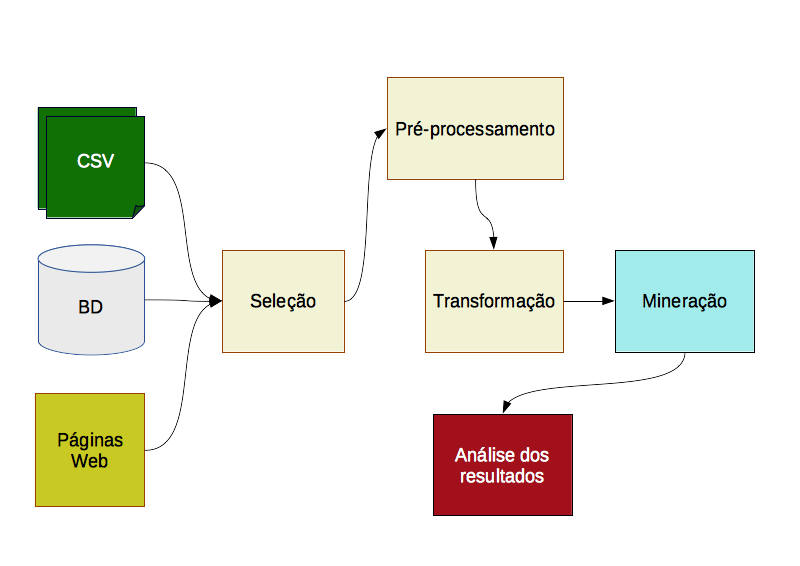
\includegraphics[scale=0.8]{imagens/kdd.png}
    \legend{Fonte: Baseado em \citeonline{Silva2010}}
  \end{center}
\end{figure}
\newpage

% ---
% Início das etapas
\subsection{Seleção dos dados}

O processo de KDD é iniciado pela etapa de seleção de dados. Este é um passo demorado e, muitas vezes, complexo, visto que um projeto pode utilizar uma ou mais fontes de dados para a seleção, e o que será coletado durante esta etapa também vai variar de acordo com o contexto do projeto. É comum que as informações a serem coletadas sejam escolhidas por um especialista no domínio do problema \cite{Boente2008}. A seleção de dados, muitas vezes, se depara com fontes que apresentam os seus dados de forma semiestruturada ou não estruturada. Neste sentido é necessário criar programas ou utilizar ferramentas que auxiliem, de maneira prática, o acesso, captura e armazenamento das informações.

É comum utilizarmos linguagens de programação para a criação de scripts que automatizam o trabalho de seleção, a exemplo da linguagem Python\footnote{\url{https://www.python.org}} \cite{Smedt2012}. Também podemos utilizar a linguagem SQL para a extração de informações já estruturadas em bases de dados consolidadas. Fica evidente, então, que esta etapa poderá utilizar uma ou mais ferramentas para a sua execução.

\subsection{Pré-processamento}

Em posse das informações coletadas na etapa anterior, a etapa de  pré-processamento é iniciada. Esta é uma etapa muito importante no processo KDD, visto que é comum realizarmos ajustes no conjunto de dados, que visam melhorar a qualidade das informações coletadas \cite{Aggarwal2015}. Ilustrações de tarefas de pré processamento são a remoção de dados redundantes e inconsistentes, identificação e avaliação de dados discrepantes, tratamento de dados ausentes, normatização para formatos de datas e obtenção de informações a partir de outras características como, por exemplo, a obtenção de idades de pessoas a partir de datas de nascimento ou nome de cidades por meio do código de endereçamento postal (CEP).

\subsection{Transformação}

Logo após a seleção e pré processamento dos dados, é preciso transformar este resultado de uma maneira que as informações estejam padronizadas para consultas posteriores. Esta etapa representa a consolidação dos últimos dois passos. Para que os algoritmos de mineração possam trabalhar em cima dos dados é necessário que durante a etapa de transformação os dados como um todo sejam convertidos para o formato adequado de acesso.

O armazenamento de dados normalmente é feito em um SGBD (Sistema gerenciador de banco de dados), mas também é possível encontrá-los  em arquivos tabulares como, por exemplo, em arquivos CSV\footnote{Formato de arquivo texto comumente empregado utilizado para a troca de dados entre aplicações, no qual cada linha corresponde a um registro e os campos são separados entre si por vírgula.} (\emph{Comma-Separated Values}). Dependendo da ferramenta utilizada para a análise dos dados, é possível que o armazenamento em um SGBD ou em arquivos CSV não seja suficiente.

Ferramentas como o Weka \cite{Hall2009} e Tensorflow\footnote{\url{https://www.tensorflow.org}} utilizam formatos de arquivos personalizados para a realização do trabalho de mineração. No caso do Weka o formato de arquivo é o \emph{attribute-relation file format} (ARFF)\footnote{\url{https://www.cs.waikato.ac.nz/ml/weka/arff.html}}, que na sua estrutura possui uma maneira própria para determinar os atributos e tipos de dados contidos. Sendo assim é possível que o formato de armazenamento e consolidação dos dados varie de acordo com a ferramenta escolhida para as etapas de análise.


\subsection{Mineração de dados}

Data mining ou mineração de dados é um processo automático ou semi automático que por meio de técnicas de exploração, busca a extração de novos padrões potencialmente úteis em grandes quantidades de dados, de modo que estes padrões não seriam facilmente descobertos a olho nu \cite{Fayyad1996,Witten2016}. O grande desafio nesta etapa é que cada conjunto de dados é único, o que dificulta a criação de ferramentas que possam ser reutilizadas em contextos diferentes. Também é possível categorizar  as tarefas de exploração dos dados como supervisionadas e não supervisionadas \cite{Aggarwal2015}. O processo de data mining pode ser dividido em quatro tipos de tarefas: associação de regras, classificação, agrupamento em conjuntos e  detecção de outliers \cite{Aggarwal2015}.

Quando estamos tentando definir o valor (por discriminação ou categorização) de uma coluna especial em um \emph{dataset} nós estamos trabalhando com uma tarefa de classificação. Quando estamos tentando definir grupos onde seus elementos se assemelham em nível de características, nós estamos trabalhando com uma tarefa de agrupamento (\emph{clustering}). Quando as linhas de um \emph{dataset} são muito diferentes das demais nós estamos trabalhando com uma tarefa de detecção de anomalias (\emph{outliers}) e, por fim, quando estamos detectando quais valores de atributos de um \emph{dataset} ocorrem juntos entre diferentes linhas nós estamos trabalhando com uma tarefa de regra de associação. Os próximos parágrafos abordam superficialmente cada tipo de tarefa de modo que seja possível distingui-las entre si.

A tarefa de regras de associação pode ser melhor entendida a partir de um contexto real da nossa sociedade. Temos como exemplo um supermercado onde o dono precisa saber quais produtos são mais comprados em conjunto (que ocorrem sempre juntos) e qual produto influencia na compra de outros produtos. Um outro exemplo seria em uma concessionária veicular onde uma quantidade de clientes que compram pneus também fazem serviços de manutenção como o alinhamento.

Segundo \citeonline{Ng1994}, “a análise em agrupamentos é uma ramificação da estatística que possibilita o agrupamento automático de um conjunto de objetos com base nas suas características e nível de semelhança". Os algoritmos de agrupamento utilizam técnicas que medem a "distância de similaridade" (e.g, Distância euclidiana e Manhattan) entre elementos \cite{Sinwar2014}. Um exemplo clássico de agrupamento envolve um conjunto de flores particionadas em três grupos distintos, onde as informações sobre cada planta remetem ao tamanho e largura das suas pétalas e sépalas. O algoritmo de agrupamento tenta adivinhar a quais grupos as flores pertencem baseado nas similaridades de seus atributos (dimensões).

A detecção de \emph{outliers} é outra tarefa inserida no domínio de Data Mining. Um outlier corresponde a uma observação que diverge das demais observações ao ponto de despertar suspeitas \cite{Chandola2009}. A técnica de detecção de \emph{outliers} utiliza a clusterização como etapa intermediária para segmentar grupos similares e assim destacar as ocorrências que divergem dos grupos caracterizados. Um exemplo clássico é o problema de detecção de transações fraudulentas em uma operadora de cartões de crédito, que busca identificar discrepâncias no comportamento de compras dos seus clientes.

Por fim, mas não menos importante, podemos nos deparar com a tarefa de classificação. Esta tarefa tem o objetivo de atribuir um rótulo para uma ou mais instâncias de um \emph{dataset} de modo que esta atribuição seja feita por meio da análise prévia de características de outras instâncias similares. Um exemplo prático pode ser visto com a classificação de doenças em níveis de intensidade (classes), onde o classificador irá se basear em dados de um \emph{dataset} como os sintomas (atributos) de cada instância da doença para formar um conhecimento que será utilizado para predizer o nível de uma nova instância de doença ainda não conhecida dentro do \emph{dataset}.

A tarefa de classificação é considerada como uma tarefa de aprendizado supervisionada, já que é preciso apresentar ao algoritmo de aprendizagem informações prévias sobre os dados como os seus atributos e classes. Do outro modo nós temos as tarefas de agrupamento, regra de associação e detecção de \emph{outliers} que são consideradas como tarefas de aprendizado não supervisionado, já que não são apresentadas ao algoritmo de aprendizagem informações para "ensinar" como a tarefa será executada perante os dados em questão \cite{Aggarwal2015}.

Este trabalho utiliza as técnicas de classificação e por isso estas serão apresentadas em detalhes na seção 2.3.


\subsection{Interpretação dos resultados}

Logo após a mineração dos dados, entramos na fase de interpretação e avaliação dos resultados obtidos.  É comum que nesta etapa os resultados da mineração sejam avaliados por um especialista no domínio do problema a fim de corroborar o conhecimento que foi minerado a partir dos dados brutos. Esta é uma fase que tende a ser realizada várias vezes durante um mesmo projeto pois é normal que as informações encontradas não sejam precisas o suficiente ou não façam sentido para o contexto do projeto nas primeiras iterações. O especialista do domínio assiste a esse processo e ajuda a reinicializar todo o processo de KDD ou parte dele sempre que necessário. Desta forma é possível que os dados e características selecionadas na primeira etapa sofram modificações, assim como a etapa de mineração de dados em si com o algoritmo escolhido para tal.

\section{Técnicas de Classificação}
Existem inúmeras técnicas de mineração descritas na literatura, muitas remetem aos quatro grande tarefas apresentados na seção anterior. Este tópico tem como intuito apresentar algoritmos de aprendizagem utilizados em técnicas de classificação, suas limitações e seus principais casos de uso.

Os algoritmos de aprendizagem de máquina podem ser chamados de classificadores quando a tarefa a ser executada é de classificação. Um classificador pode ser entendido como uma função que recebe informações de entrada e, a partir do processamento dessas informações, produz uma saída conhecida como modelo \cite{Fayyad1996}. Este processo é conhecido como treinamento.

O classificador pode trabalhar com tarefas onde as opções de classes para treinamento e predição variam entre duas ou mais, desta maneira a tarefa de classificação pode ser binária ou multiclasse (ou multinomial) \cite{Aggarwal2015}.

A classificação binária remete à tarefa onde o algoritmo precisa aprender sobre duas classes, geralmente as classes dizem respeito a uma indicação de Positivo e Negativo. Um exemplo de classificação binária é quando o algoritmo precisa determinar se um paciente está ou não com uma doença específica. Já um problema multiclasse remete à tarefa onde o algoritmo precisa aprender sobre como classificar uma instância mediante a escolha entre três ou mais opções de classes. Classificar uma doença por meio de vários níveis de risco é uma tarefa de classificação multiclasse.

Os modelos de classificação são produzidos a partir de informações estatísticas, lógicas e padrões resultantes do processamento dos dados de entrada\footnote{\url{https://docs.microsoft.com/en-us/sql/analysis-services/data-mining/mining-models-analysis-services-data-mining}}, e estes dados são as instâncias de um \emph{dataset} e os seus atributos. É possível utilizar a mesma fonte de dados para treinar vários modelos diferentes de classificação. Algoritmos como Naive Bayes \cite{Mccallum1998}, \emph{Support Vector Machines} (SVM) \cite{Meyer2017} e árvores de decisão \cite{Schmid2013} resultarão em modelos distintos, cada um com suas características, pontos fortes e fracos. A escolha de qual algoritmo utilizar vai depender, por exemplo, do contexto do problema, tamanho do \emph{dataset} e nível de desbalanceamento das classes (desproporção entre o número de exemplos de cada classe).

Antes da criação de um modelo de dados é preciso selecionar quais instâncias de um \emph{dataset} serão utilizadas para treinamento do algoritmo. Existem técnicas específicas para esta necessidade, sendo as mais conhecidas: a \emph{holdout} e a \emph{k-fold Cross-validation} \cite{Kohavi1995}.

O método \emph{holdout} é o mais simples dos dois mencionados, pois consiste em segmentar o \emph{dataset} em subconjuntos de treino e de teste, onde os segmentos são mutuamente excludentes. Historicamente são utilizadas as proporçòes de $\frac{2}{3}$ do \emph{dataset} para treino e de $\frac{1}{3}$ para teste \cite{Kohavi1995}.

Um dos problemas do método \emph{holdout} é que normalmente a seleção das instâncias se torna enviesada se as classes estiverem em desproporção nas partições ou se a forma de seleção das instâncias não for feita de uma maneira aleatória e sem repetição. É comum que as partições dos conjuntos de treino e teste sejam feitas com um método chamado de estratificação, onde a estratificação é responsável por montar os grupos com a seleção aleatória das instâncias a partir do \textit{dataset}. Desta forma a seleção das instâncias não segue uma sequência linear e os grupos podem manter a proporção de instâncias.

Levando em consideração um \emph{dataset} que possui a mesma quantidade de elementos para duas classes diferentes e, se o holdout utilizado não for estratificado, a partição de treino é realizada na proporção de $\frac{2}{3}$. Esta, por sua vez, possuirá mais elementos de uma classe do que de outra (desproporção ou desbalanceamento) o que poderá afetar no resultado do treinamento \cite{Witten2016}.

O método \emph{k-fold} consiste em segmentar o conjunto de dados em K grupos (\emph{folds}) mutuamente excludentes, onde o treinamento do algoritmo será feito com k-1 \emph{folds} e o \emph{fold} restante será utilizado para teste, havendo um rodízio na formação dos conjuntos de treino e testes para garantir que todos os grupos participem do conjunto de treino e de testes. \citeonline{Kohavi1995} demonstra que a escolha de $k = 10$ é razoavelmente adequada para a grande maioria dos problemas, visto que o resultado da classificação não é melhorado de forma significativa para grandes valores de K, o que não justificaria o esforço computacional utilizado para o treinamento.

É necessário observar que o método \emph{k-fold} é computacionalmente mais caro que o método \emph{Holdout} já que o algoritmo será treinado k vezes, contudo esta abordagem diminui o viés dos dados entregues para o algoritmo de treinamento, o que, consequentemente gera melhores resultados de classificação \citeonline{Kohavi1995}.


\section{Ferramentas de Suporte à Análise de Dados}

A partir da evolução da Computação e da popularização da Ciência de Dados, ferramentas cada vez mais completas tem sido criadas para oferecer o suporte necessário para as etapas da análise de dados. Atualmente algumas das ferramentas mais utilizadas para este fim são a Weka \cite{Hall2009}, a linguagem de programação R\footnote{\url{https://www.r-project.org}} e a linguagem de programação Python\footnote{\url{https://www.python.org}}.

\subsection{Weka}

Segundo \citeonline{Frank2016}, Weka é uma coleção de algoritmos de aprendizagem de máquina para tarefas de \textit{data mining}. Os algoritmos podem ser aplicados diretamente a um \textit{dataset} usando a interface do Weka Explorer ou podem ser invocados a partir de um código Java\footnote{\url{https://www.java.com/}} (Weka API - Application Programming Interface). Weka provê suporte para tarefas de  pré-processamento, classificação, regressão, regras de associação e visualização de resultados. A ferramenta Weka foi escrita na linguagem  Java. Diferentemente do Python e R, o Weka oferece uma interface gráfica pronta para uso, assim é possível realizar todas as operações da mineração de dados por meio desta interface (Figura \ref{fig:weka}).

\begin{figure}[htb]
  \caption{\label{fig:weka}Weka GUI Interface}
  \begin{center}
    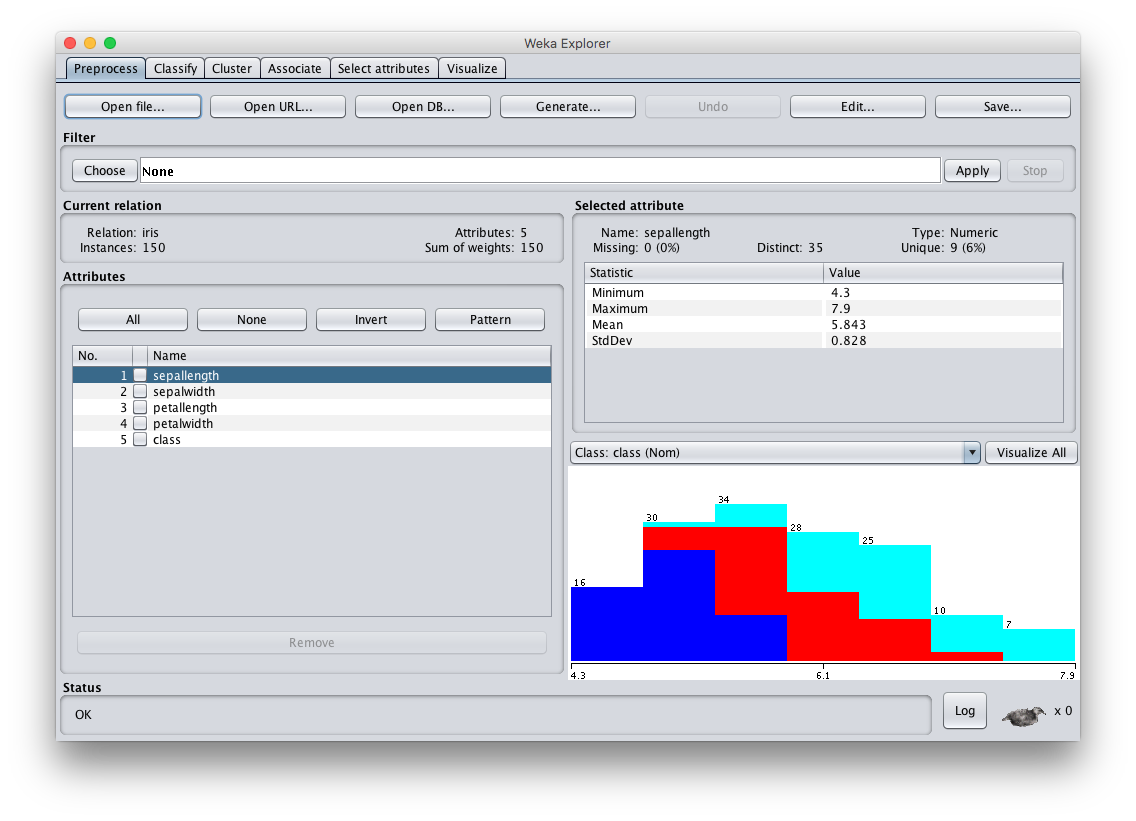
\includegraphics[scale=0.4]{imagens/weka.png}
    \legend{Fonte: \citeonline{Hall2009}}
  \end{center}
\end{figure}
\newpage

A Figura \ref{fig:weka} exibe a interface gráfica da ferramenta Weka, onde é possível ver os menus disponíveis para realizar as tarefas de classificação,  agrupamento e associação. Figura \ref{fig:weka} também exibe as informações sobre o \textit{dataset} e seus atributos.

\subsection{Linguagem R}
R é um software livre que combina um linguagem de programação e um ambiente de desenvolvimento integrado para a realização de cálculos estatísticos, visualização de gráficos e execução de rotinas de código armazenadas em \textit{script} \cite{Team2018}.

A linguagem disponibiliza um REPL (\textit{read-eval-print-loop}) para a execução de comandos de maneira rápida e fácil, sendo possível criar e invocar funções, criar e carregar \textit{datasets} e criar e carregar modelos estatísticos. Por se tratar de um software \textit{open source}\footnote{\url{https://opensource.org}}, R conta com uma quantidade expressiva de colaboradores, estes, por sua vez, disponibilizam extensões para o ecossistema da linguagem. R também conta com um grupo de desenvolvedores dedicados para a linguagem desde 1997, o que traz mais segurança para que mais pessoas e empresas invistam na sua utilização.


\subsection{Python}

Python é uma linguagem de programação interpretada de propósito geral, imperativa, orientada a objetos, funcional, de tipagem dinâmica e forte\footnote{\url{https://www.python.org/doc/essays/blurb/}}. É  linguagem de alto nível que é fundamentada na priorização do esforço do programador acima do esforço computacional.

Diferentemente do Weka e da linguagem R, Python não foi criada com o intuito de servir à computação estatística e gráfica, porém, por sua capacidade de extensão, os desenvolvedores colaborativos criaram módulos que conversam com outras linguagens de programação como FORTRAN\footnote{\url{https://web.fe.up.pt/~aarh/pc/PC-capitulo2.pdf}} e C\footnote{\url{https://docs.python.org/2/extending/extending.html}} o que tornou possível a criação de algoritmos eficientes para a análise de dados. Atualmente é possível encontrar muitos módulos para a análise de dados e visualização dos resultados para Python.

\section{Métricas para Avaliação}

Mensurar o desempenho de um algoritmo durante o processo de mineração é de suma importância. É preciso estabelecer métricas e parâmetros reproduzíveis para que haja a comparação de resultados entre diferentes algoritmos. É por meio das métricas de avaliação que poderemos analisar e ter \textit{insights} sobre os dados, ou seja, saberemos quais algoritmos possuem melhor desempenho para o caso em questão.

As medidas de \textit{precision} (precisão), \textit{recall} (\textit{sensitivity}, sensitividade ou cobertura) e \textit{f-measure} são comumente empregadas para avaliar o desempenho de algoritmos de classificação \cite{Powers2011}. A especificidade  (\textit{specificity} ou  \textit{inverse-recall}) também pode ser utilizada. Estes parâmetros são utilizados em pelo menos uma métrica de avaliação da Matriz de confusão.

\subsection{Matriz de confusão}

A matriz de confusão não é um método propriamente dito para medição do desempenho de um algoritmo de classificação, contudo, auxilia na visualização da classificação \cite{Deng2016} e entendimento do comportamento do classificador. A matriz gera uma tabulação com as informações sobre a classificação, dessa forma fica mais fácil analisar qual foi o comportamento da mineração.

Para entender a saída de dados da matriz de confusão é preciso conhecer o significado das siglas apresentadas na Tabela 1, estas são: Verdadeiros Positivos (TP), Falsos Positivos (FP), Verdadeiros Negativos (TN) e Falsos Negativos (FN) \cite{Powers2011}, vale lembrar que após a classificação os termos serão substituídos por números que representam as instâncias classificadas.

A Tabela \ref{tab:confusion} é um exemplo de uma matriz de confusão para a classificação com duas classes de exemplo, uma positiva e outra negativa. O parâmetro TP representa a quantidade de verdadeiros positivos que foram classificados corretamente para a  classe positiva, o parâmetro TN representa a quantidade de verdadeiros negativos que foram classificados corretamente para a classe negativa. O parâmetro FP representa a quantidade de instâncias que foram classificadas incorretamente para a classe positiva (foram classificadas como positiva mas eram da classe negativa) e o parâmetro FN representa a quantidade de instâncias que foram classificadas incorretamente para a classe negativa (foram classificadas como negativa mas eram da classe positiva) \cite{Powers2011}.

\begin{table}[h]
	\caption{\label{tab:confusion}Matriz de confusão}
	\begin{center}
	\begin{tabular}{c|c}
		\hline 
		\textbf{TP} & FN \\ 
		\hline
		FP & \textbf{TN} \\ 
		\hline 
	\end{tabular} 
	\legend{Fonte: O autor}
	\end{center}
\end{table}

Logo após gerarmos a tabulação com as informações sobre a classificação, é  interessante calcular o quão eficiente foi o treinamento. A partir desse momento levamos em consideração pelo menos três métricas utilizadas na recuperação de informação \cite{Buttcher2016} para realizar a avaliação do algoritmo de aprendizagem: \textit{Recall}, \textit{Precision}, \textit{Specificity}.

\textit{Precision} (precisão) é a proporção de casos preditos como positivos e que são de fato reais positivos, sendo assim estamos medindo a capacidade do algoritmo em classificar as instâncias do \textit{dataset} corretamente para a classe positiva.

\begin{equation}
Precision  = \frac{TP}{TP + FN}
\end{equation}

\textit{Recall} (\textit{sensitivity}) é a proporção de casos que são reais positivos e que foram corretamente classificados como tal, ou seja, estamos medindo a capacidade do nosso algoritmo de classificar os verdadeiros positivos para um conjunto de dados.

\begin{equation}
Recall  = \frac{TP}{TP + FP}
\end{equation}


A \textit{Specificity} (especificidade) é a proporção de casos preditos como negativos e que são de fato reais negativos. Com esta métrica nós estamos analisando a capacidade do algoritmo em prever os casos ditos reais negativos (TN). Diferentemente do \textit{Precision} e \textit{Recall}, quando a \textit{Specificity} é analisada, a intenção é focar na classificação dos ditos casos negativos, visto que em determinados casos como na Medicina é importante validar os casos que são verdadeiros negativos (pessoas que não possuem uma doença por exemplo) \cite{Holzinger2014}.

\begin{equation}
Specificity  = \frac{TN}{TN + FN}
\end{equation}

Quanto maior a proporção para estes três casos, melhor o algoritmo teria se saído durante a classificação. Por fim, podemos calcular a \textit{Balanced Accuracy} (Precisão balanceada) para a nossa matriz de confusão, que nos dará a média entre as proporções de casos verdadeiros positivos e verdadeiros negativos.

\begin{equation}
Balanced Accuracy  = \frac{Recall + Specificity}{2}
\end{equation}

\textit{F-measure}, ou como às vezes é chamada \textit{F-score}, é a média ponderada do \textit{Recall} e \textit{Precision}. É uma função herdada da Recuperação de Informação (\textit{Information Retrieval}) onde o \textit{Recall} é a frequência em que documentos relevantes são selecionados por um sistema (Sensitividade) e o \textit{Precision} é quantidade de vezes que os documentos são preditos estão corretos \cite{Powers2014}. \textit{F-measure} combina o \textit{Recall} e o \textit{Precision} em uma única medida na busca da efetividade para a recuperação de informação. De uma maneira mais geral o \textit{F-measure} foca nas informações relevantes para a classe positiva e não leva em consideração as informações da especificidade. A sua fórmula pode ser vista a seguir.

\begin{equation}
F  = \frac{2 * (Precision * Recall)}{Precision + Recall}
\end{equation}


\section{Trabalhos Relacionados}

A descoberta de conhecimento em base de dados tem sido utilizada como matéria prima para a obtenção de informações relevantes e como apoio para a tomada de decisão. Alguns estudos utilizam a mineração de dados na área da saúde para realizar triagem de pacientes em hospitais, predizer surtos de doenças em determinadas áreas e detectar doenças como câncer de pele.

\citeonline{Khoo2015} utilizou métodos de predição com a regressão linear para prever os casos de dengue em um intervalo de 16 dias no ano de 2011 na cidade de Kuala Lumpur. Este estudo demonstra como é possível aplicar as técnicas do KDD em um conjunto de dados históricos sobre a dengue juntamente com fatores ambientais como chuvas, temperaturas e vegetação para criar um modelo estatístico capaz de predizer a quantidade de casos em um intervalo pré determinado. Com isso o estudo demonstra como foi possível ajudar a comunidade ao redor da University of Malaya (UM) com a tomada de medidas de precaução.

A mineração de dados e a extração de conhecimento foi utilizada por \citeonline{Funchal2016} a fim de criar uma ferramenta capaz de classificar pacientes em grupos de risco durante o processo de triagem de um hospital universitário no estado do Rio Grande do Sul. \citeonline{Funchal2016} demonstra que após a análise de quatro estudos de caso foi possível determinar que as enfermeiras que cuidavam da triagem dos pacientes não obedeciam uma lógica definida para a classificação manual, o que resultava em grandes filas para o atendimento.

No que se refere à criação de algoritmos para classificação e detecção de estágios de doenças, \citeonline{Gutman2016} demonstram um caso abordado durante um desafio no simpósio internacional sobre imagens biomédicas propôs a criação de um \textit{dataset} contendo 900 imagens de cânceres de pele em vários estágios onde os algoritmos propostos pelos participantes selecionaram-nas, utilizaram-nas e classificaram-nas de acordo com cada classe e estágio da doença.

Todos estes trabalhos utilizam técnicas de mineração de dados para obter informações sobre o contexto da Medicina, os trabalhos de \citeonline{Funchal2016,Gutman2016} são os que mais se assemelham do nosso conteúdo deste trabalho, eles demonstram como é possível criar ferramentas capazes de ajudar na busca de informações de forma automatizada contudo nenhuma delas tratou em gerar formas simplificadas de acesso ao resultado do processo de mineração. O próximo capítulo demonstra o processo e etapas de desenvolvimento das atividades realizadas neste trabalho.
\chapter{Atividades desenvolvidas}

Este capítulo apresenta as atividades realizadas para a construção de um classificador binário capaz de identificar padrões de sintomas de doenças e categorizá-los  em enfermidades do tipo Dengue ou Chikungunya. Uma aplicação web também foi desenvolvida com o intuito de utilizar o modelo de classificação para que fosse possível gerar novas predições por meio de um \textit{browser} e exibir o resultado em páginas HTML (\textit{HyperText Markup Language}).

\section{Informações sobre as doenças}

\citeonline{laoprasopwattana2012differential} e \citeonline{lee2012simple} alegam que  a distinção entre casos de Dengue e Chikungunya é difícil de ser feita de forma eficaz apenas por observação porque os sintomas e sinais são bastante similares, sendo assim, é necessário realizar exames clínicos para obter um diagnóstico satisfatório. Nesse sentido, o uso de uma sistema computacional de apoio à decisão pode ser útil, por exemplo, para realizar a triagem inicial de pacientes em um hospital de maneira mais rápida e efetiva.

Existem pelo menos dois tipos de exames que podem ser utilizados para detecção de Dengue. São eles: o RT-PCR (\textit{Reverse transcription polymerase chain reaction}) e NS1 ELISA \cite{verma2016evaluation}. Os dois exames possuem características distintas para a detecção do vírus da dengue, no Brasil o exame que utiliza o NS1 Elisa é realizado por meio do Sistema Único de Saúde (SUS) desde agosto de 2017\footnote{\url{http://pesquisa.in.gov.br/imprensa/jsp/visualiza/index.jsp?jornal=1&pagina=56&data=10/08/2017}}. \citeonline{mata2014} realizaram um estudo comparativo entre os exames de teste rápido do tipo NS1 ELISA a fim de detectar a precisão de cada um. O estudo concluiu que a precisão dos exames pode variar entre 55,8 a 83,4\%, o que pode culminar na alta equivocada de pacientes. O valor destes exames pode variar de R\$ 13,00 a R\$ 28,00.

\citeonline{Cecilia2015} demonstram em seu estudo um exame do tipo RT-PCR capaz de detectar dengue e chikungunya com taxas de assertividade de 95\% a 100\% respectivamente. Diferentemente dos exames utilizados pelo SUS, o RT-PCR é mais caro que um semelhante como o NS1 ELISA e também necessita de melhores aparatos laboratoriais \cite{verma2016evaluation}.

\citeonline{Huang2013} demonstram a perda de eficácia para os exames do tipo NS1 ELISA à medida que os dias de infecção passam e isto é um agravante no caso dos usuários do SUS já que o manual de diagnóstico e manejo para a dengue\footnote{\url{http://bvsms.saude.gov.br/bvs/publicacoes/dengue_diagnostico_manejo_adulto_crianca_3ed.pdf}} recomenda a realização do exame clínico a partir do sexto dia de início dos sintomas.

Diante das dificuldades e limitações existentes na triagem de pacientes e, considerando que nem sempre exames podem ser realizados rápida e eficazmente, busca-se, por meio de sinais e sintomas identificados, realizar a classificação proposta neste trabalho. A metodologia aplicada é explicada a seguir.

\section{Metodologia}
Sabendo que os sinais e sintomas apresentados pelas duas doenças são semelhantes e que a distinção entre as duas por meio de uma observação empírica é dificultada por tais características, foi proposta uma hipótese de investigação. A hipótese definida foi:

\textit{É possível realizar a classificação entre duas doenças com sinais e sintomas similares, descritos apenas de forma binária como "sim ou não", de modo que a probabilidade de acerto seja igual ou superior a 80\%?}

A porcentagem de 80\% para a precisão de acerto foi definida levando em consideração os exames clínicos existentes, onde os exames mais acessíveis possuem média semelhante para a detecção das duas doenças.

Para a execução deste trabalho as etapas a seguir foram realizadas:

\begin{enumerate}[label=\roman*]
 \item Levantamento do estado da arte;
 \item Obtenção de dados sobre Dengue e Chikungunya;
 \item Compreensão dos dados sobre Dengue e Chikungunya;
 \item Seleção, pré-processamento, integração e persistência dos dados;
 \item Estudo de algoritmos de classificação;
 \item Aplicação de algoritmos de classificação;
 \item Avaliação dos resultados;
 \item Construção de uma aplicação que permita a interação com o classificador
\end{enumerate}


\section{Dados sobre as arboviroses}

A concepção do modelo de classificação - objeto deste trabalho - utilizou um conjunto de dados de pacientes da rede pública de atendimento do estado da Paraíba, concedidos pela Secretaria da Saúde do Estado da Paraíba (SES-PB). Os dados fornecem informações sobre os pacientes com suspeita ou com a confirmação de Dengue e Chikungunya no ano de 2016.

Os dados, disponibilizados em formato de arquivo CSV, compreendem entre 156 e 159 atributos de informação (colunas no arquivo), para dengue e chikungunya respectivamente. Os atributos variam desde a localidade de moradia do paciente até o resultado de exames realizados. A Figura \ref{fig:csvses} exibe um fragmento do \textit{dataset}, onde é possível observar que existem instâncias com dados não informados como também é possível observar o tipo de informação que as colunas possuem (o valor 1 representa SIM e o valor 2 representa NÃO).

\begin{figure}[htb]
  \caption{\label{fig:csvses}Fragmento de informação sobre doenças}
  \begin{center}
    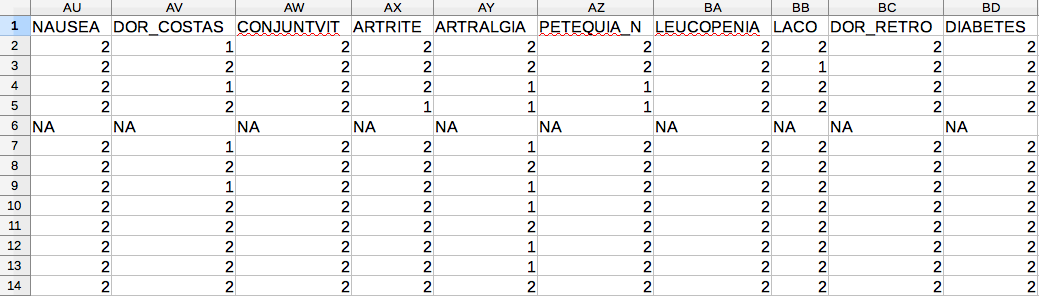
\includegraphics[width=\textwidth]{imagens/fragmentodosdados.png}
    \legend{Fonte: SES-PB}
  \end{center}
\end{figure}

Inicialmente, foi necessário analisar o conjunto de metadados para entender o contexto das informações inerentes ao domínio das arboviroses (Dengue e Chikungunya), visto que, por algumas vezes, os nomes dos atributos não eram claros o suficiente para expressar o seu significado. Para contornar este problema, utilizamos os metadados fornecidos pelo portal de dados abertos da cidade do Recife\footnote{\url{http://dados.recife.pe.gov.br/dataset/rede-de-saude-municipal}}, que também permite acesso a um conjunto dados sobre as doenças investigadas na cidade do Recife. A Figura \ref{fig:metadados} exibe um fragmento dos metadados fornecidos pelo portal, onde é possível observar que as informações também não são conclusivas, porém é de grande ajuda a detecção do grupo de informação ao qual um atributo pertence.

\begin{figure}[htb]
  \caption{\label{fig:metadados}Fragmento dos metadados sobre sinais e sintomas das doenças}
  \begin{center}
    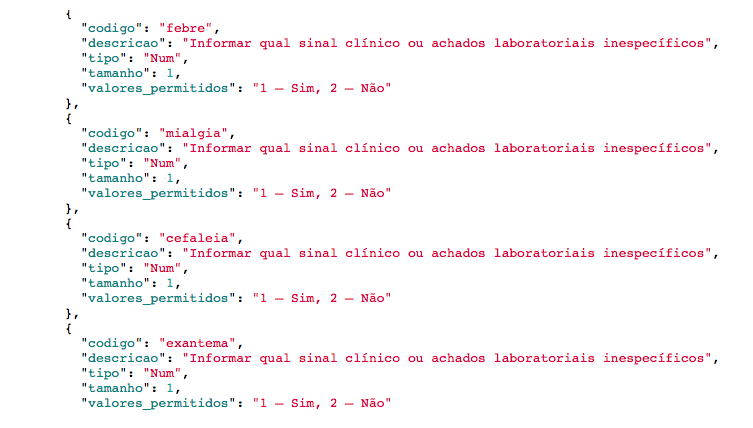
\includegraphics[width=\textwidth]{imagens/fragmentodosmetadados.png}
    \legend{Fonte: Portal de dados abertos do Recife}
  \end{center}
\end{figure}
\newpage

\section{Preparação do conjunto de dados}

As etapas de seleção, pré-processamento e transformação do KDD foram aplicadas aos dados fornecidos pela SES-PB. Na fase de seleção, foram removidos do \textit{dataset} os dados sobre outras doenças fora do contexto deste trabalho como também os atributos que em nada contribuíram durante a fase de mineração, como, por exemplo, a cidade do paciente.

Durante a etapa de pré-processamento, foi necessário efetuar a normalização de datas para um formato único. Também foram removidas instâncias que não possuíam as informações completas sobre o quadro de sinais e sintomas das doenças. Nesta etapa também foram retiradas do \textit{dataset} as instâncias que estavam marcadas como casos descartados ou inconclusivos. Inicialmente o \textit{dataset} contava com 58.657 instâncias sobre os pacientes e, após a etapa de pré-processamento, 17.205 instâncias restaram. De uma média de 157 atributos apenas 21 foram mantidos. Estes atributos são os sinais e sintomas dos pacientes para cada doença (Tabela \ref{tab:21colunas}).

\begin{table}[h]
\begin{center}
\caption{\label{tab:21colunas}Colunas selecionadas após processamento}

\begin{tabular}{c|c|c|c}
\hline 
Febre & Mialgia & Cefaleia & Exantema \\ 
\hline 
Vômito & Náusea & Dor nas costas & Conjuntivite \\ 
\hline 
Artrite & Artralgia & Auto Imune & Petéquia \\ 
\hline 
Leucopenia & Prova do laço & Dor Retro-orbitária & Diabetes \\ 
\hline 
Doenças renais & Hipertensão & Ácido péptico & • \\ 
\hline 
\end{tabular} 
\legend{Fonte: O autor}

\end{center}
\end{table}
\newpage

Na etapa  de transformação, os dados foram mantidos em dois formatos distintos para posterior utilização: CSV e ARFF. Para realizar a transformação do arquivo CSV em um arquivo ARFF foi construído um script na linguagem Python capaz de produzir um arquivo ARFF a partir dos dados e metadados de um arquivo CSV.

O Quadro \ref{quadro:arff} exibe um fragmento do arquivo de tipo ARFF criado a partir das informações do arquivo CSV. É possível observar que a estrutura do arquivo é bem definida com espaços para nomear o \textit{dataset}, registrar os atributos, marcar os tipos de dados para cada atributo e registrar as informações propriamente ditas sobre o conjunto de dados, ou seja, seus valores.

\begin{quadro}
\caption{\label{quadro:arff}Fragmento do arquivo ARFF}
\begingroup
    \fontsize{10pt}{9pt}\selectfont
    \begin{verbatim}  
@RELATION dengue-chikungunya

@ATTRIBUTE FEBRE Numeric
@ATTRIBUTE MIALGIA Numeric
@ATTRIBUTE CEFALEIA Numeric
@ATTRIBUTE EXANTEMA Numeric
@ATTRIBUTE VOMITO Numeric
@ATTRIBUTE NAUSEA Numeric
@ATTRIBUTE DOR_COSTAS Numeric
@ATTRIBUTE CONJUNTVIT Numeric
@ATTRIBUTE ARTRITE Numeric
@ATTRIBUTE ARTRALGIA Numeric
@ATTRIBUTE PETEQUIA_N Numeric
@ATTRIBUTE LEUCOPENIA Numeric
@ATTRIBUTE LACO Numeric
@ATTRIBUTE DOR_RETRO Numeric
@ATTRIBUTE DIABETES Numeric
@ATTRIBUTE HEMATOLOG Numeric
@ATTRIBUTE HEPATOPAT Numeric
@ATTRIBUTE RENAL Numeric
@ATTRIBUTE HIPERTENSA Numeric
@ATTRIBUTE ACIDO_PEPT Numeric
@ATTRIBUTE AUTO_IMUNE Numeric
@ATTRIBUTE CLASS {chikungunya,dengue}

@DATA
0,1,0,1,0,0,1,0,0,1,0,0,0,0,0,0,0,0,0,0,0,chikungunya
1,1,1,1,1,1,0,0,0,1,0,0,0,1,0,0,0,0,0,0,0,dengue
1,1,1,1,0,0,1,0,0,1,0,0,0,0,0,0,0,0,0,0,0,dengue
    \end{verbatim}  
\endgroup
\legend{Fonte: O autor}
\end{quadro}
\newpage

\section{O processo de classificação e algoritmos utilizados}

A tarefa de classificação foi escolhida para ser analisada no processo de mineração de dados porque nós já havíamos iniciado outro processo de classificação com dados similares, dessa forma existia uma certa familiaridade com tal tarefa. Com os dados previamente consolidados, o processo de criação do classificador pôde ser iniciado. Nesta etapa a hipótese foi investigada exaustivamente, também foram analisados os parâmetros de sensitividade e especificidade resultantes de cada classificação. Os três algoritmos escolhidos para a realização da classificação foram Naive bayes, \textit{Support Vector Machine} (SVM) e \textit{Classification and Regression Trees} (CART). Estes são algoritmos bastante utilizados em áreas como agricultura, medicina e geologia \cite{dong2014nonlinear}.

Assim que a etapa de transformação dos dados foi finalizada, o processo de classificação pôde ser iniciado. A linguagem R foi utilizada para treinar e testar os modelos de classificação. Para treinamento dos algoritmos foram utilizadas as 17.205 instâncias resultantes da fase de pré-processamento dos dados (100\% dos dados), e foi utilizado o método \textit{k-fold Cross-Validation} com o número de \textit{fold} definido em 10 ($k = 10$). As próximas seções (3.5.1, 3.5.2, 3.5.3, 3.5.4) demonstram o processo de classificação para cada um dos algoritmos escolhidos para este experimento, bem como seu respectivo desempenho, e a Seção 3.5.5 condensa as informações apresentadas com uma análise final para os resultados.

\subsection{Naive Bayes}
O classificador Naive Bayes é um dos mais utilizados no aprendizado de máquina por causa da sua simplicidade, velocidade para treinamento e capacidade em aprender sobre problemas complexos \cite{dong2014nonlinear,zhang2004optimality,chakrabarti2002mining}. Trata-se de um algoritmo fundamentado no teorema de Bayes para classificação probabilística. O teorema determina a probabilidade de acontecimento para uma classe de acordo com as observações de dados anteriores \cite{Aggarwal2015}. Desta forma, é possível atualizar a probabilidade de um evento após investigar as evidências sobre o mesmo. O teorema recebe este nome não só por causa do seu descobridor (Thomas Bayes) mas também por ser considerado ingênuo (\textit{naive}) pela sua suposição de que todas as variáveis de um problema são independentes condicionalmente, sendo assim o acontecimento de um evento não deve influenciar na ocorrência de outros conjuntos de eventos para outras variáveis.

O primeiro teste de classificação foi realizado utilizando o algoritmo Naive Bayes, onde os parâmetros para treinamento foram os 21 sinais e sintomas mostrados na Tabela \ref{tab:21colunas}  para as duas doenças. A matriz de confusão pode ser vista no Quadro \ref{quadro:naivematriz1}.

\begin{quadro}
\caption{\label{quadro:naivematriz1}Matriz de confusão do algoritmo Naive Bayes}
\begingroup
    \fontsize{10pt}{9pt}\selectfont
    \begin{Verbatim}[commandchars=\\\{\}]
      Confusion Matrix and Statistics
                    Reference
       Prediction      dengue  chikungunya
       dengue            \textbf{9244}       5389
       chikungunya       791        \textbf{1781}
                                         
               Accuracy : 0.6408         
                 95% CI : (0.6336, 0.648)
     \textbf{Sensitivity/Recall} : 0.9212         
            \textbf{Specificity} : 0.2484         
      \textbf{Balanced Accuracy} : 0.5848
              F-measure : 0.7494        
         
       'Positive' Class : dengue 
       'Negative' Class : chikungunya
  
    \end{Verbatim}  
\endgroup
\legend{Fonte: O autor}
\end{quadro}
\newpage

Por meio do Quadro \ref{quadro:naivematriz1} é possível observar que a precisão balanceada foi de 58,48\%, ou seja, o algoritmo foi capaz de acertar 58,48\% das vezes para o nosso conjunto de dados. É importante ressaltar que apenas essa medida não é suficiente para informar se um algoritmo é bom ou ruim para o conjunto dos dados, é preciso observar também as medidas como \textit{sensitivity} e \textit{specificity}.

É possível observar no Quadro \ref{quadro:naivematriz1} que o algoritmo Naive Bayes foi muito enfático para determinar quais instâncias pertenciam ao conjunto da Dengue. Conforme resultado da medida de sensitividade (\textit{sensitivity} ou \textit{recall}), em 92,12\% das instâncias o algoritmo classificou corretamente os casos de dengue. Entretanto a medida de especificidade (\textit{specificity}) demonstra que o algoritmo acertou apenas 24,84\% dos casos para a Chikungunya. De uma maneira geral o algoritmo não obteve a performance necessária para validar a hipótese do trabalho e demonstrou uma certa tendência para classificar as instâncias como Dengue, o que, por sua vez, pode ser um aspecto perigoso quando tratamos de identificar doenças.

\subsection{\textit{Classification and Regression Trees}}

O CART representa uma árvore de decisão binária e recursiva de particionamento capaz de processar valores numéricos e nominais como atributos e classes \cite{steinberg2009cart}. O processo de particionamento começa com um nó central que posteriormente é dividido em mais dois nós filhos, e os particionamentos seguem até que não haja mais a possibilidade para divisões, o CART permite a criação de várias árvores de decisão a fim de eleger uma árvore que possua o melhor balanço entre o \textit{overfitting} e o \textit{underfitting}. Informações mais detalhadas sobre o CART podem ser vistos em \citeonline{breiman2017classification}.

Assim como no processo de classificação com o Naive Bayes, foram utilizados os 21 atributos. O Quadro \ref{quadro:cart1} demonstra o resultado da classificação utilizando o CART.


\begin{quadro}
\caption{\label{quadro:cart1}Matriz de confusão do algoritmo CART}
\begingroup
    \fontsize{10pt}{9pt}\selectfont
    \begin{Verbatim}[commandchars=\\\{\}]
      Confusion Matrix and Statistics
                    Reference
       Prediction      dengue  chikungunya
       dengue            \textbf{7981}       2835
       chikungunya       2054        \textbf{4335}
                                         
               Accuracy : 0.7158         
                 95% CI : (0.709, 0.7226)
     \textbf{Sensitivity/Recall} : 0.7953         
            \textbf{Specificity} : 0.6046         
      \textbf{Balanced Accuracy} : 0.7000
              F-measure : 0.7655        
         
       'Positive' Class : dengue 
       'Negative' Class : chikungunya
  
    \end{Verbatim}  
\endgroup
\legend{Fonte: O autor}
\end{quadro}

É possível observar que a precisão balanceada é de 70.00\%, ou seja, 11.52\% mais alta que o Naive Bayes, entretanto também precisamos observar as outras estatísticas derivadas do processo. Para a classificação de instâncias com o rótulo real de Dengue (sensitividade), o algoritmo obteve uma precisão de 79.53\%, representando uma redução de 12.59\% em comparação com o Naive Bayes. A classificação de instâncias com o rótulo de Chikungunya (especificidade) obteve uma performance de 60.46\%, o que representa 35.62\% acima do Naive Bayes.

De uma maneira geral, o CART obteve uma performance consideravelmente superior ao Naive Bayes. Com a precisão média em 70.00\%, o CART não atingiu a performance mínima esperada pela hipótese do trabalho.

\subsection{\textit{Support Vector Machine}}

O \textit{Support Vector Machine} (SVM) é um algoritmo de aprendizagem de máquina, do tipo supervisionado, que cria vetores em um espaço de hiperplanos por meio dos atributos dos dados de treinamento a fim de criar uma separação entre instâncias de classes diferentes \cite{rebentrost2014quantum}. No caso da classificação, a separação é feita em exemplos positivos e negativos. A idéia básica é encontrar o hiperplano de separação ideal entre os exemplos positivos e negativos.

A Figura \ref{fig:svm} demonstra um exemplo para a classificação de instâncias onde o hiperplano é do tipo linear, é possível observar a margem de separação entre os grupos de cada classes, como também é possível observar os vetores de suporte que cruzam as instâncias no plano (X, Y).

\begin{figure}[htb]
  \caption{\label{fig:svm}Hiperplanos de separação e Vetores de suporte }
  \begin{center}
    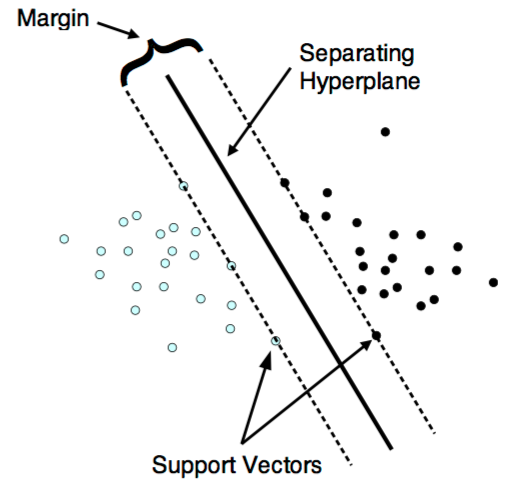
\includegraphics[scale=0.4]{imagens/svm.png}
    \legend{Fonte: \citeonline{Meyer2017}}
  \end{center}
\end{figure}
\newpage

O hiperplaneiro ideal pode ser obtido maximizando a margem entre dois hiperplanos paralelos \cite{qi2013robust}. Esta é uma técnica  poderosa e muito utilizada para gerar modelos de classificação \cite{Meyer2017}. Mais informações sobre o embasamento teórico e funcionamento do algoritmo podem ser encontradas no trabalho de \citeonline{cortes1995support}.

Assim como nos exemplos com o Naive Bayes e CART, foi gerado um modelo de classificação utilizando o SVM. A O Quadro \ref{quadro:svm1} exibe a matriz de confusão e as estatísticas de classificação. É possível observar que a precisão média é ligeiramente superior (2.35\%) à média apresentada pelo CART, a sensitividade é 6.28\% inferior e a precisão em classificar a Chikungunya é 10.99\% maior.

\begin{quadro}
\caption{\label{quadro:svm1}Matriz de confusão do algoritmo SVM}
\begingroup
    \fontsize{10pt}{9pt}\selectfont
    \begin{Verbatim}[commandchars=\\\{\}]
      Confusion Matrix and Statistics
                    Reference
       Prediction      dengue  chikungunya
       dengue            \textbf{7351}       2047
       chikungunya       2684        \textbf{5123}
                                         
               Accuracy : 0.725         
                 95% CI : (0.7183, 0.7317) 
     \textbf{Sensitivity/Recall} : 0.7325         
            \textbf{Specificity} : 0.7145         
      \textbf{Balanced Accuracy} : 0.7235
              F-measure : 0.7565        
         
       'Positive' Class : dengue 
       'Negative' Class : chikungunya
  
    \end{Verbatim}  
\endgroup
\legend{Fonte: O autor}
\end{quadro}


\subsection{Experimentação aplicando a técnica de Seleção de Atributos}

Como foi discutido anteriormente, os sinais e sintomas apresentados pelos pacientes são muito parecidos. Dois pacientes com os mesmos sintomas podem ter doenças diferentes (entre Dengue e Chikungunya). Este fenômeno é conhecido na mineração de dados como overlapping ou sobreposição de classes \cite{xiong2010classification}.

A sobreposição de classes dificulta o trabalho do algoritmo de classificação, visto que fica mais difícil identificar corretamente a qual classe uma instância pertence. Como \citeonline{martin2009suitability} sugerem, existem técnicas específicas para tratar este problema, algumas das técnicas sugeridas são a seleção de atributos específicos por correlação\footnote{É uma técnica verifica quais atributos possuem uma correlação alta ou moderada em relação a classe e uma baixa correlação entre os outros atributos \citeonline{hall1999correlation}.} e ganho de informação\footnote{O ganho de informação técnica que visa selecionar os atributos de um \textit{dataset} que mais contribuem para o aumento do desempenho de um algoritmo de predição.}.


A fim de observar mais de perto o domínio dos dados nós realizamos experimentos com a seleção de atributos utilizando a ferramenta Weka. Foi aplicada a técnica de seleção de atributos por meio da medida de ganho de informação. O Weka criou um ranking com os atributos mais relevantes para a predição da classe das doenças e, ao seu término,  7 dos 21 atributos foram selecionados, onde, em teoria, os sintomas descartados não devem impactar negativamente no desempenho dos classificadores. Os sintomas selecionados podem ser vistos na Tabela \ref{tab:7colunas}. 

Logo após a seleção dos atributos mais relevantes, o processo de classificação foi reiniciado com os mesmos algoritmos dos testes iniciais. Nos testes com o algoritmo Naive Bayes foi detectada uma melhora de performance de 4.54\%, o algoritmo CART obteve uma performance de 68.78\% (uma perda de 1.22\%), e o algoritmo SVM obteve uma performance de 68.39\%, uma perda de 3.96\% em sua precisão média. As matrizes de confusão podem ser consultadas no \textbf{Apêndice A}.


\begin{table}[h]
\begin{center}
\caption{\label{tab:7colunas}Sinais e sintomas selecionados para classificação}

\begin{tabular}{c|c|c|c}
\hline 
Artralgia & Dor nas costas & Conjuntivite & Artrite \\ 
\hline 
Náuseas & Exantema & Hipertensão & • \\ 
\hline 
\end{tabular} 

\legend{Fonte: O autor}

\end{center}
\end{table}
\newpage

\subsection{Análise geral da classificação}

Com o fim do processo de classificação foi possível quantificar qual algoritmo obteve uma melhor precisão balanceada para o nosso conjunto de dados. O algoritmo de \textit{Support Vector Machine} obteve a melhor performance nas primeiras rodadas de teste, e o algoritmo CART obteve a melhor performance após a seleção de atributos. A Figura \ref{fig:precisoesbalanceadas} exibe as precisões médias de classificação para as duas iterações.

\begin{figure}[htb]
  \caption{\label{fig:precisoesbalanceadas}Precisão balanceada para classificação}
  \begin{center}
    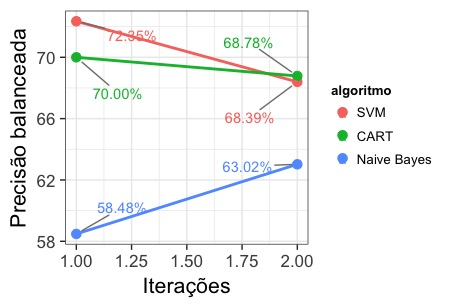
\includegraphics[scale=0.7]{imagens/atributos_selecao_desempenho_linhas.jpeg}
    \legend{Fonte: O Autor}
  \end{center}
\end{figure}

De uma maneira geral, os três algoritmos não obtiveram a medição  mínima de desempenho para validar a hipótese. Entendemos que a natureza do problema de classificação abordado neste trabalho não demanda uma solução trivial, e é necessário especializar o processo de classificação direcionado às particularidades do problema.

Fatores como o desbalanceamento do \textit{dataset} e \textit{overlapping} de classes impactaram diretamente os resultados apresentados, outros fatores como atributos binários não ajudam para a detecção da borda de decisão. Para clarificar este entendimento podemos ter como exemplo a possibilidade de que o sinal de febre seja mais acentuado em uma doença que em outra, sendo assim, esta característica poderia vir a ajudar numa melhor classificação. A obtenção de atributos adicionais e relevantes para identificação  das  duas doenças poderá ajudar na melhoria do desempenho  dos classificadores. Ainda assim, é necessário levar em consideração que mesmo com mais dados há o risco da borda que separa estas duas doenças não ser suficientemente clara para as técnicas selecionadas para a classificação.

\section{Aplicação Web (ArboML)}

Após a criação do classificador foi iniciado o processo de especificação e implementação de uma aplicação que permita a interação com o mesmo e que tornasse fácil o acesso e visualização do resultado. Foi escolhido implementar uma interface que pudesse ser acessada por meio dos \textit{browsers} e da internet e que não fosse preciso instalar nada no dispositivo de acesso.

A Figura \ref{fig:arboml} exibe a implementação da interface de classificação sendo acessada por um navegador como também sinais e sintomas selecionados e o resultado da classificação ao lado. O funcionamento da interface é bem simples: o usuário pode selecionar quais sinais e sintomas são apresentados, e o resultado da predição é atualizado em tempo real. Toda a comunicação entre o classificador e a interface ArboML é feito via protocolo HTTP com chamadas assíncronas a um servidor que mantém o classificador online.

\begin{figure}[htb]
  \caption{\label{fig:arboml}ArboML}
  \begin{center}
    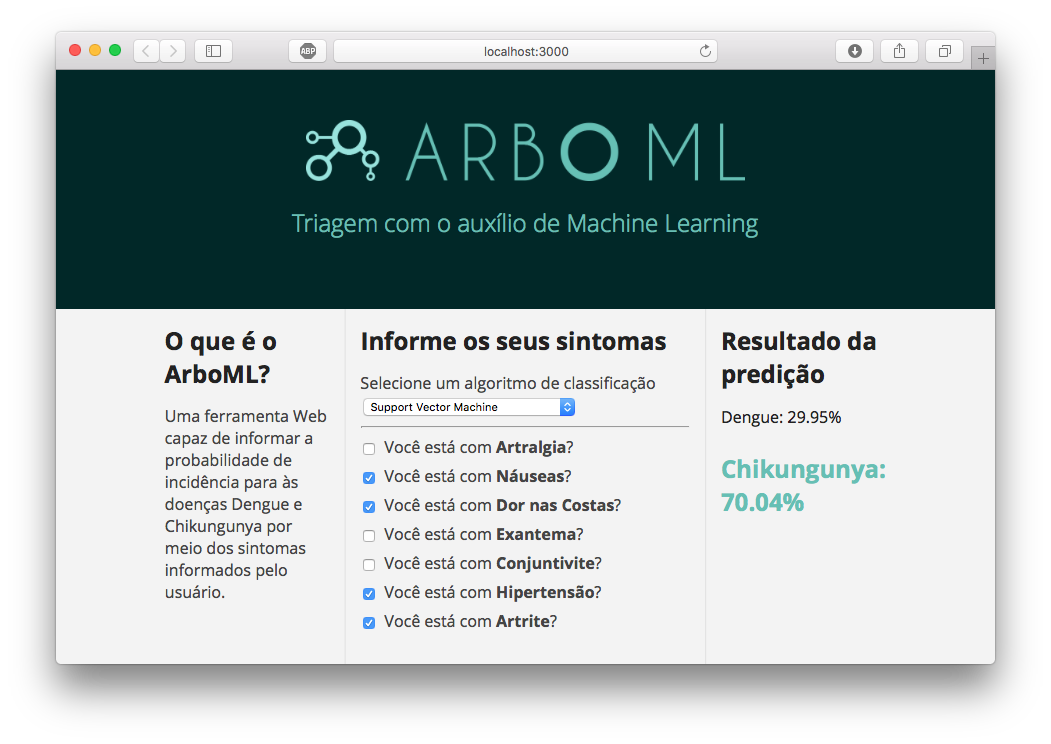
\includegraphics[scale=0.46]{imagens/arboML.png}
    \legend{Fonte: O Autor}
  \end{center}
\end{figure}
\newpage

A ArboML foi implementada utilizando tecnologias como HTML, \textit{Cascading Style Sheets} (CSS) e JavaScript onde o principal foco é o JavaScript que é responsável em fazer as chamadas ao servidor do classificador. A princípio, a ArboML tem o intuito de apresentar  apresentar o resultado da classificação de forma simples, clara e objetiva ao usuário final. A precisão da classificação da doença é determinada pela avaliação de desempenho dos classificadores. Não faz parte do escopo deste trabalho uma avaliação qualitativa da usabilidade da ArboML, tendo em vista que foram detectadas necessidades de trabalhos futuros para aprimoramento da metodologia utilizada neste trabalho, cujo foco se concentra nas atividades de mineração em si. A aplicação e seus aspectos de usabilidade serão futuramente estendidas.

A Figura \ref{fig:api} demonstra a arquitetura de acesso aos classificadores por meio de uma API que utiliza o protocolo HTTP para expor a interface de acesso aos classificadores produzidos neste trabalho.

\begin{figure}[htb]
  \caption{\label{fig:api}Arquitetura de interação com o classificador}
  \begin{center}
    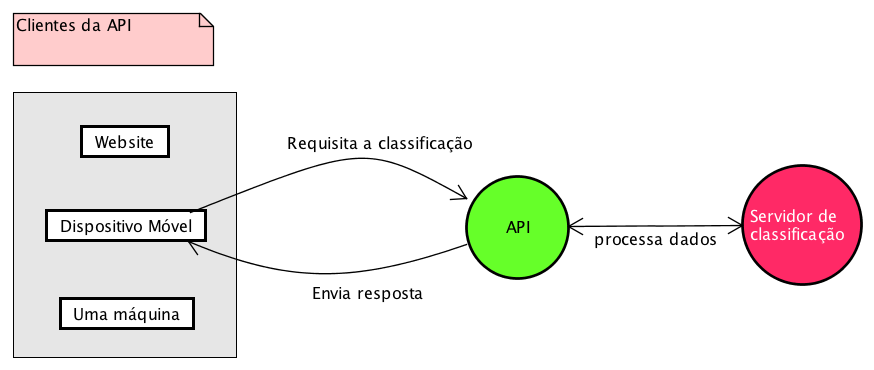
\includegraphics[scale=0.7]{imagens/api-diagram.png}
    \legend{Fonte: O Autor}
  \end{center}
\end{figure}
\newpage

\chapter{Considerações finais}

Neste trabalho foi mostrado um modelo de classificação para Dengue e Chikungunya desenvolvido durante um projeto de pesquisa de inovação tecnológica. O modelo de classificação é utilizado por uma aplicação web para prover uma interface visual e clara do processo de classificação aos usuário final, possibilitando assim a sua utilização de maneira efetiva.


\section{Contribuições}

A aplicação web (ArboML) cria uma interface de acesso por meio da internet para um classificador de Dengue e Chikungunya que utiliza os sinais e sintomas apresentados por um ser humano para elencar o índice de probabilidade para cada uma das doenças. A interface disponibiliza um questionário simples que serve de guia para colher dados sobre o estado físico de uma pessoa de modo que o tempo de feedback entre as perguntas e respostas seja o menor possível.

Também podem ser consideradas contribuições do projeto de pesquisa todo o processo que envolveu o ETL dos dados originais e a análise e entendimento das informações sobre as doenças. Além destes, foram realizados um processo de extração de informações referentes às precipitações de chuvas no estado da Paraíba, um processo para a criação de um modelo de regressão capaz de prever o aumento ou diminuição dos casos relacionados às arboviroses no estado da Paraíba (por município, região e microrregião) e uma aplicação de visualização de forma gráfica das predições em formato de mapas de calor.

\section{Dificuldades encontradas}

A principal dificuldade encontrada durante a realização deste trabalho tem uma relação muito profunda com manuseio dos dados disponibilizados pela SES-PB. Estes dados são advindos do dia a dia de trabalho de centenas de pessoas no estado da Paraíba o que possibilita a criação de um problema na qualidade de coleta. A falta de dados mais precisos,  balanceados e  normalizados impactou diretamente em todo o processo de KDD. Foi necessário a realização de um processo dispendioso, em termos de tempo, para que os dados fossem preparados para o treinamento do algoritmo de classificação.

Além do problema relacionado à qualidade dos dados, foi detectado um problema muito característico das doenças do escopo deste trabalho: seus sinais e sintomas muito semelhantes afetam a acurácia da classificação, o suficiente para não se chegar a um patamar de concorrência com os exames clínicos. Este fator revela a importância de abordar o problema de classificação considerando esta particularidade.

\section{Trabalhos futuros}

Para trabalhos futuros nós gostaríamos de propor uma investigação mais profunda sobre o relacionamento dos sintomas das doenças e sua classificação por meio de outras técnicas de classificação como o \textit{deep learning}\footnote{\url{http://neuralnetworksanddeeplearning.com/chap6.html}}, \textit{Cost Sensitive Learning} e \textit{Active Learning} \cite{krishnamurthy2017active} e também outra técnica como \textit{Clustering}. Também se faz necessário a realização de experimentos em conjuntos de dados maiores e de diferentes regiões do Brasil o que possibilitaria a construção de uma base mais homogênea para a população brasileira e com mais informações para o treinamento do algoritmo.

% ---
% Referências
%- \bibliography{referencias}
% ----------------------------------------------------------
% ELEMENTOS PÓS-TEXTUAIS
% ----------------------------------------------------------
\postextual
% ----------------------------------------------------------

% ----------------------------------------------------------
% Referências bibliográficas
% ----------------------------------------------------------
\bibliography{referencias}

% ----------------------------------------------------------
% Apêndices
% ----------------------------------------------------------
% ---
% Inicia os apêndices
% ---
\begin{apendicesenv}

% Imprime uma página indicando o início dos apêndices
\partapendices

% ----------------------------------------------------------
\chapter{Resultados das classificações}
% ----------------------------------------------------------

\begin{quadro}
\caption{\label{quadro:naive2}Matriz de confusão do algoritmo Naive bayes com seleção de atributos}
\begingroup
    \fontsize{10pt}{9pt}\selectfont
    \begin{Verbatim}[commandchars=\\\{\}]
      Confusion Matrix and Statistics
                    Reference
       Prediction      dengue  chikungunya
       dengue            \textbf{8738}       4376
       chikungunya       1297        \textbf{2794}
                                         
               Accuracy : 0.6703         
                 95% CI : (0.6632, 0.6773)     
     \textbf{Sensitivity/Recall} : 0.8708         
            \textbf{Specificity} : 0.3897         
      \textbf{Balanced Accuracy} : 0.6302
         
       'Positive' Class : dengue 
       'Negative' Class : chikungunya
  
    \end{Verbatim}  
\endgroup
\legend{Fonte: O autor}
\end{quadro}


\begin{quadro}
\caption{\label{quadro:cart2}Matriz de confusão do algoritmo CART com seleção de atributos}
\begingroup
    \fontsize{10pt}{9pt}\selectfont
    \begin{Verbatim}[commandchars=\\\{\}]
      Confusion Matrix and Statistics
                    Reference
       Prediction      dengue  chikungunya
       dengue            \textbf{7064}       2354
       chikungunya       2971        \textbf{4816}
                                         
               Accuracy : 0.6905         
                 95% CI : (0.6835, 0.6974)      
     \textbf{Sensitivity/Recall} : 0.7039         
            \textbf{Specificity} : 0.6717         
      \textbf{Balanced Accuracy} : 0.6878
         
       'Positive' Class : dengue 
       'Negative' Class : chikungunya
  
    \end{Verbatim}  
\endgroup
\legend{Fonte: O autor}
\end{quadro}


\begin{quadro}
\caption{\label{quadro:naive2}Matriz de confusão do algoritmo SVM com seleção de atributos}
\begingroup
    \fontsize{10pt}{9pt}\selectfont
    \begin{Verbatim}[commandchars=\\\{\}]
      Confusion Matrix and Statistics
                    Reference
       Prediction      dengue  chikungunya
       dengue            \textbf{7181}       2493
       chikungunya       2854        \textbf{4677}
                                         
               Accuracy : 0.6892         
                 95% CI : (0.6822, 0.6961)      
     \textbf{Sensitivity/Recall} : 0.7156         
            \textbf{Specificity} : 0.6523         
      \textbf{Balanced Accuracy} : 0.6839
         
       'Positive' Class : dengue 
       'Negative' Class : chikungunya
  
    \end{Verbatim}  
\endgroup
\legend{Fonte: O autor}
\end{quadro}


\end{apendicesenv}
% ---



\end{document}